\documentclass[english,floatsintext,]{apa6}

\usepackage{amssymb,amsmath}
\usepackage{ifxetex,ifluatex}
\usepackage{fixltx2e} % provides \textsubscript
\ifnum 0\ifxetex 1\fi\ifluatex 1\fi=0 % if pdftex
  \usepackage[T1]{fontenc}
  \usepackage[utf8]{inputenc}
\else % if luatex or xelatex
  \ifxetex
    \usepackage{mathspec}
    \usepackage{xltxtra,xunicode}
  \else
    \usepackage{fontspec}
  \fi
  \defaultfontfeatures{Mapping=tex-text,Scale=MatchLowercase}
  \newcommand{\euro}{€}
\fi
% use upquote if available, for straight quotes in verbatim environments
\IfFileExists{upquote.sty}{\usepackage{upquote}}{}
% use microtype if available
\IfFileExists{microtype.sty}{\usepackage{microtype}}{}

% Table formatting
\usepackage{longtable, booktabs}
\usepackage{lscape}
% \usepackage[counterclockwise]{rotating}   % Landscape page setup for large tables
\usepackage{multirow}		% Table styling
\usepackage{tabularx}		% Control Column width
\usepackage[flushleft]{threeparttable}	% Allows for three part tables with a specified notes section
\usepackage{threeparttablex}            % Lets threeparttable work with longtable

% Create new environments so endfloat can handle them
% \newenvironment{ltable}
%   {\begin{landscape}\begin{center}\begin{threeparttable}}
%   {\end{threeparttable}\end{center}\end{landscape}}

\newenvironment{lltable}
  {\begin{landscape}\begin{center}\begin{ThreePartTable}}
  {\end{ThreePartTable}\end{center}\end{landscape}}




% The following enables adjusting longtable caption width to table width
% Solution found at http://golatex.de/longtable-mit-caption-so-breit-wie-die-tabelle-t15767.html
\makeatletter
\newcommand\LastLTentrywidth{1em}
\newlength\longtablewidth
\setlength{\longtablewidth}{1in}
\newcommand\getlongtablewidth{%
 \begingroup
  \ifcsname LT@\roman{LT@tables}\endcsname
  \global\longtablewidth=0pt
  \renewcommand\LT@entry[2]{\global\advance\longtablewidth by ##2\relax\gdef\LastLTentrywidth{##2}}%
  \@nameuse{LT@\roman{LT@tables}}%
  \fi
\endgroup}


  \usepackage{graphicx}
  \makeatletter
  \def\maxwidth{\ifdim\Gin@nat@width>\linewidth\linewidth\else\Gin@nat@width\fi}
  \def\maxheight{\ifdim\Gin@nat@height>\textheight\textheight\else\Gin@nat@height\fi}
  \makeatother
  % Scale images if necessary, so that they will not overflow the page
  % margins by default, and it is still possible to overwrite the defaults
  % using explicit options in \includegraphics[width, height, ...]{}
  \setkeys{Gin}{width=\maxwidth,height=\maxheight,keepaspectratio}
\ifxetex
  \usepackage[setpagesize=false, % page size defined by xetex
              unicode=false, % unicode breaks when used with xetex
              xetex]{hyperref}
\else
  \usepackage[unicode=true]{hyperref}
\fi
\hypersetup{breaklinks=true,
            pdfauthor={},
            pdftitle={Demonstrating opportunities of visualisation and network analysis in physical activity and its determinants: Baseline associations in the Let's Move It trial},
            colorlinks=true,
            citecolor=blue,
            urlcolor=blue,
            linkcolor=black,
            pdfborder={0 0 0}}
\urlstyle{same}  % don't use monospace font for urls

\setlength{\parindent}{0pt}
%\setlength{\parskip}{0pt plus 0pt minus 0pt}

\setlength{\emergencystretch}{3em}  % prevent overfull lines

\ifxetex
  \usepackage{polyglossia}
  \setmainlanguage{}
\else
  \usepackage[english]{babel}
\fi

% Manuscript styling
\captionsetup{font=singlespacing,justification=justified}
\usepackage{csquotes}
\usepackage{upgreek}

 % Line numbering
  \usepackage{lineno}
  \linenumbers


\usepackage{tikz} % Variable definition to generate author note

% fix for \tightlist problem in pandoc 1.14
\providecommand{\tightlist}{%
  \setlength{\itemsep}{0pt}\setlength{\parskip}{0pt}}

% Essential manuscript parts
  \title{Demonstrating opportunities of visualisation and network analysis in
physical activity and its determinants: Baseline associations in the
Let's Move It trial}

  \shorttitle{Visualisation and network analysis in physical activity}


  \author{Matti T. J. Heino\textsuperscript{1,2*}, Eiko Fried\textsuperscript{3}, Reijo Sund\textsuperscript{1,2}, Ari Haukkala\textsuperscript{1}, Keegan Knittle\textsuperscript{1}, Katja Borodulin\textsuperscript{1}, Antti Uutela\textsuperscript{1}, Vera Araujo-Soares\textsuperscript{1}, Falko Sniehotta\textsuperscript{1}, Tommi Vasankari\textsuperscript{1}, Nelli Hankonen\textsuperscript{1}, NULL, NULL, \& NULL}

  % \def\affdep{{"", "", "", "", "", "", "", "", "", "", "", "", "", ""}}%
  % \def\affcity{{"", "", "", "", "", "", "", "", "", "", "", "", "", ""}}%


  \authornote{
    Trial Registration Number: ISRCTN10979479. Registered retrospectively:
    31.12.2015
    
    Correspondence concerning this article should be addressed to Matti T.
    J. Heino, . E-mail:
    \href{mailto:matti.tj.heino@gmail.com}{\nolinkurl{matti.tj.heino@gmail.com}}
  }


  \abstract{Background: Let's Move It is a cluster-randomised controlled trial
evaluating a novel theory-based intervention, which aimed to reduce
sedentary behaviour (SB) and increase physical activity (PA) among older
adolescents in vocational schools, by targeting environmental and
psychosocial determinants of the phenomena. This paper describes the
characteristics of the LMI baseline cohort in both arms, and explores
the possibilities for visually presenting such data, making use of
recent developments in software and network analyses. We provide a
template for researchers to apply these tools to other data. Methods: At
baseline, 1123 adolescents in 57 classes in 6 school units participated
in the study. Data were gathered with 7-day accelerometry, bioimpedance
measures and questionnaires, which were used to measure health status,
activity behaviours, and potential constructs mediating the effect of
the intervention on outcomes. Data were visualised e.g.~combining ridge
plots and diamond plots; network analysis was used to investigate
relations between psychosocial variables and outcomes. Results: The
participants were 16-49 years old (M = 18.5, SD = xx, Md = 18.0). On
average, they engaged in moderate-to-vigorous PA xx (SD = xx, Md = xx)
and SB xx minutes daily and xx breaks in SB. Several variables differ
among the four educational tracks, but not across intervention and
control groups. Conclusion: The usage of behaviour change techniques
Autonomous motivation . Comparability to similar populations.. We have
also shown benefits of presenting such data visually, and encourage
researchers to routinely make the extensive analyses and descriptions
they have produced, available in website supplements.}
  \keywords{exercise, physical activity, school-based intervention, behaviour
change, sedentary behaviour \\

    \indent Word count: X
  }





\usepackage{amsthm}
\newtheorem{theorem}{Theorem}[section]
\newtheorem{lemma}{Lemma}[section]
\theoremstyle{definition}
\newtheorem{definition}{Definition}[section]
\newtheorem{corollary}{Corollary}[section]
\newtheorem{proposition}{Proposition}[section]
\theoremstyle{definition}
\newtheorem{example}{Example}[section]
\theoremstyle{definition}
\newtheorem{exercise}{Exercise}[section]
\theoremstyle{remark}
\newtheorem*{remark}{Remark}
\newtheorem*{solution}{Solution}
\begin{document}

\maketitle

\setcounter{secnumdepth}{0}



\newpage

\section{Background}\label{background}

Declining physical activity (PA) and increasing sedentary behaviour (SB)
are costly and growing concerns for public health, especially for
individuals with low socioeconomic status (SES) (Elgar et al., 2015,
Dieleman et al. (2018)). Patterns of low PA among adults begin earlier
in life. Among children, the evidence regarding psychosocial predictors
of PA and SB, and especially objectively measured activity, is quite
clear (CITE KATJA? ). As there is evidence that the declines in PA and
increases in SB are already evident in childhood and adolescence (P.
Husu, Vähä-Ypyä, \& Vasankari, 2016; Mäkelä et al., 2016), there is a
need for further research on to how to improve PA and SB among
adolescents.

As adolescents spend a significant amount of their time in schools,
schools provide a promising opportunity for PA interventions REF(van
Sluijs et al., 2008). The Let's Move It intervention aimed to reduce SB
and increase PA among adolescents in vocational schools; developed using
stakeholder input and co-creation with target group representatives, as
well as behavioural science theory and empirical evidence (N. Hankonen
et al., 2017b; S.-T. Hynynen et al., 2016). The effectiveness of Let's
Move It has now been tested in a cluster-randomised controlled trial.
Contrary to typical school-based interventions with uniform study
populations, this trial was carried out in vocational schools with
different educational tracks, differences between which may be important
to making accurate conclusions in the trial evaluation phase.

The programme theory (explicated in REF: DEVELOPMENT; see
\href{mailto:also@rogersUsingProgrammeTheory2008a}{\nolinkurl{also@rogersUsingProgrammeTheory2008a}},
and G. F. Moore et al. (2015), p.~32) for changing PA and SB was
hypothesised to be slightly different for PA and SB. In order to engage
in PA, one needs to have a conscious effort and self-regulatory capacity
to make use of the opportunities, such as planning for active times and
overcoming barriers to exercise. In the intervention, one of the key
emphases in helping adolescents change their PA was to help them
understand and use techniques to manage their motivation and behaviour
(see also N. Hankonen et al. (2017a)). Assessing what participants do to
advances our understanding of what people themselves can do to in
attempts to change their behaviour. To date, there is little systematic
theorising on how the use of these techniques link to each other, and it
would be important to understand these interlinkages empirically. The
model for SB, on the other hand, is more driven by environmental
opportunities and incentives, such as having the option of standing up
during class.

In order to change moderate-to-vigorous-intensity PA, a central
component of the intervention targeted autonomous motivation, social
cognitions, as well as participants' skills to use behaviour change
techniques to self-regulate motivation and behaviour (Hankonen et al,
unpublished manuscript). To change SB, or specifically, to reduce total
SB as well as introduce breaks in SB, the program aimed to change the
school environment by training teachers in providing more active
teaching and altering physical choice architecture in classrooms (Köykkä
et al, accepted) . The intervention included also poster campaign in
schools and a website, as well as materials to target community actors
and parents (N. Hankonen et al., 2016). More information of the content
of the intervention and the development of it is reported elsewhere
(Hankonen et al 2017 NELLI?), Hankonen et al unpublished manuscript).
The mediators postulated by the program theory included behavioural
beliefs (outcome expectations, descriptive norms, intention,
self-efficacy/perceived behavioural control), autonomous and controlled
motivation, environmental opportunities, action and coping planning, and
behaviour change technique (BCT) use. Key hypotheses regarding students'
PA change have been registered OSF (\url{https://osf.io/tb8fu/}). It has
long been a standard recommendation for quantitative analyses to
investigate data visually as a core precursor of conducting statistical
analyses (Tukey 1977 Exploratory Data Analysis; Cleveland 1993
Visualizing data). However, in social and life sciences, such
visualizations have rarely been shared in publications. Information
about data are usually limited to means and standard deviations, which
presents at best limited information about the variables of interest.
Medians, modes, skewness and kurtosis provide helpful additional
information, but can still hide important distributional properties.

Successful communication of important information includes additional
means of communication to flooding readers with unintuitive numerical
point values or easily reified bound estimates, such as confidence
intervals. Visualizing data is imperative, because it allows for
communicating large amounts of information-and the associated
uncertainty-in an accessible format, without requiring extensive
mathematical background from the reader. Unfortunately, traditional word
count limits in scientific publications, along with a stringent
limitations on the number of tables and figures that can be included,
have prohibited researchers sharing data visualization. When researchers
extend work on previous findings of others, they thus may not know that
they are working with inadequately complete information; this has direct
implications to the recent crisis of confidence in the reproducibility
and replicability of research findings (REF).

Three recent developments allow a different approach. First, many
journals now allow for publication of supplementary online materials,
which circumvents both word and figure restrictions of traditional
manuscripts. Second, statistical software such as R (REF) has recently
become increasingly mainstream among applied researchers, opening the
door for a wide variety of data visualisation techniques. Third, novel
statistical methods in social and health psychology, such as
psychological network analysis, may help in understanding relationships
of variables by making better use of visual representations of their
associations.

In summary, by describing the characteristics of the Let's Move It
baseline cohort, the current paper aims to (1) provide a strong
rationale for the urgency of data visualization, discuss its advantages,
and recent developments in scientific publishing, statistical software,
and statistical models that enable researchers to use data visualization
tools more easily and efficiently; (2) provides a detailed visualization
of the LMI trial baseline data, with focus on psychosocial correlates
and hypothesised mediators of the intervention effect on
moderate-to-vigorous physical activity; and (3) provides all code to use
as a template for and delivers the information in a format which only
necessitates a web browser to access.

\section{Methods}\label{methods}

The study has been described earlier in N. Hankonen et al. (2016). In
brief, the study was a cluster-randomised controlled trial of a complex
multi-level intervention based in Finnish vocational schools. The
consenting participants answered an electronic survey, underwent
bioimpedance measurement and were instructed to wear an accelerometer
for seven consecutive days.

Study design, screening and recruitment

Five schools providing four educational tracks; 1. Practical Nurse
(Nur), 2. Hotel, Restaurant and Catering (HRC), 3. Business and
Administration (BA), and 4. Information and Communications Technology
(IT) were recruited. Schools were paired so that there would be matching
numbers of students from each educational track for both members of the
pair. Blinded randomization by a statistician without knowledge of
pairs, track or schools was then conducted so that a random member of
each pair was selected as case school, the other as control school
(details reported in N. Hankonen et al. (2016)). Participants were blind
to randomisation at baseline.

\subsection{Measures}\label{measures}

The measurements have been previously described in N. Hankonen et al.
(2016), and all individual items of the scales are available in the
supplementary file {[}MATTI TODO{]}. Thus, we will present these
baseline measures only briefly.

\subsubsection{Primary outcome
variables}\label{primary-outcome-variables}

The primary outcome for PA was moderate-to-vigorous intensity physical
activity (MVPA). It was measured by accelerometry and self-reports.
Primary outcomes for sedentary behaviour (SB) were measured by the
accelerometer. They included time spent sitting or lying down, and the
number of times sitting was interrupted during a day.

\emph{Self-reported MVPA.} Self-reported MVPA was measured with two
questions in accordance with the NordPAQ measurement (Fagt et al.,
2012). The first question asked participants about the number of days in
which they did more than 30 minutes of MVPA during the last week, the
other asked about the overall amount of MVPA (in hours) during the
previous week.

\emph{Accelerometer-measured MVPA.} Within one week after responding to
the questionnaire, students were given an accelerometer to be worn for
seven consecutive days. The hip-worn accelerometer (Hookie AM 20,
Traxmeet Ltd, Espoo, Finland) using a digital triaxial acceleration
sensor (ADXL345; Analog Devices, Norwood MA) was attached to a flexible
belt and participants were instructed to wear the belt around their
right hip for seven consecutive days during waking hours, except during
shower and other water activities. The acceleration signal was collected
at 100 Hz sampling frequency, ±16 g acceleration range and 0.004 g
resolution. PA-parameters were based on mean amplitude deviation (MAD)
of the resultant acceleration analysed in 6s epochs (Henri
VÃ\textcurrencyhÃ\textcurrency-YpyÃ\textcurrency, Vasankari, Husu, Suni,
\& Sievänen, 2015b). The MAD values were then converted to metabolic
equivalent (MET) values (Henri
VÃ\textcurrencyhÃ\textcurrency-YpyÃ\textcurrency et al., 2015a). The
epoch-wise MET values were further smoothed by calculating 1min
exponential moving average {[}**TOMMI CHECK if 1min moving avg or 6s
epoch{]} exponential moving average**{]}. Using the smoothed MET values
total PA was classified in terms of energy consumption covering MET
values higher than 1.5 and moderate-to-vigorous PA (MVPA) covering MET
values equal to or higher than 3 (Henri
VÃ\textcurrencyhÃ\textcurrency-YpyÃ\textcurrency et al., 2015a, 2015b).

\emph{Sedentary behaviour.} According to the definition of SB (Tremblay
et al., 2017), time spent in sitting and reclining positions were
combined to indicate SB, whereas standing was analysed separately as
another form of stationary behaviour. Body postures were recognized from
the raw acceleration data by employing both direction and intensity
information from all three measurement axes. The recognition was based
on the low intensity of movement (\textless{}1.5 MET) and the
accelerometer orientation in relation to identified upright position
(angle for posture estimation, APE) calculated at the end of each 6 s
epoch (H. VÃ\textcurrencyhÃ\textcurrency-YpyÃ\textcurrency, Husu, Suni,
Vasankari, \& Sievänen, 2018).

\subsubsection{Theoretical predictors of
PA}\label{theoretical-predictors-of-pa}

The mediators postulated by the program theory included behavioural
beliefs (outcome expectations, descriptive norms, intention,
self-efficacy/perceived behavioural control), autonomous and controlled
motivation, opportunities, action- and coping planning, and behaviour
change technique (BCT) use. Participants were allowed to skip questions,
and scales were computed as means of all items where responses were
available. Items and scales are available in the supplemental file.

\subsubsection{Statistical analysis}\label{statistical-analysis}

We used RStudio (RStudio Team, 2016) running R (Version 3.5.0; R Core
Team, 2018) for all our analyses and figures.

We used psychological network analysis to estimate and visualize
relations among items. Such networks contain nodes (variables) and edges
(statistical relationships between variables). We used state-of-the-art
network models that estimate conditional dependence relations among a
set of items, which can be interpreted akin to partial correlations. An
edge between two variables implies that they are related after
controlling for all other items; the absence of an edge implies that the
two items are conditionally independent.

Specifically, we demonstrate use of a Mixed Graphical Model that is the
appropriate network model for our data. This model uses regularization,
a procedure that has been shown to help recover the true network
structure in data in case the data were simulated under a network model.
Regularization has the goal to avoid estimating spurious relationships
among items (i.e.~false positive relations), and results in a
parsimonious network structure. The regularization technique used here
is the Least Absolute Shrinkage and Selection Operator (LASSO;
Tibshirani (1996)), which shrinks all edges and sets very small edges to
exact zero. A paper that explains lasso regularization in network models
in detail can be found elsewhere (Epskamp \& Fried, 2018).

Network analysis has recently shown promise in many fields such as
social psychology (Dalege, Borsboom, Harreveld, Waldorp, \& Maas, 2017;
Dalege et al., 2016), personality (Mõttus \& Allerhand, 2017),
intelligence (Van Der Maas, Kan, Marsman, \& Stevenson, 2017),
psychopathology (Fried et al., 2017), and empathy research (Briganti,
Kempenaers, Braun, Fried, \& Linkowski, 2018), and is beginning to be
applied for health behaviours on a broader scale. Several helpful
tutorial papers aimed at empirical researchers working in psychology are
available (Dalege, Borsboom, van Harreveld, and van der Maas (2017);
Epskamp and Fried (2018); Epskamp, Borsboom, and Fried (2016);
Costantini et al. (2015); Costantini et al. (2017){]}.

Network models applied to between-subjects data at one time-point can be
useful for describing health psychological data, as well as facilitating
group-level hypothesis generation regarding which parts of the system
are central for a problem at hand (\enquote{Moving forward.}).
Identifying these determinants of importance can thus supplement
traditional structural equation modeling (SEM) approaches, while dealing
with some possibly problematic approaches to SEM (REF Borsboom
theoretical status of latent variables, Bringmann 2018, but see also
Bringmann \& Eronen, 2018). Network analysis naturally entails its own
set of assumptions. As with any model, it does not make sense to include
variables which can be thought to be embedded in each other. For
example, it is difficult to justify argue that there is no conceptual
overlap between positive outcome expectations and autonomous motivation.
Behaviour change technique usage seems less problematic in this regard.

\section{Findings}\label{findings}

Table \ref{tab:demographics-table} shows the main demographic variables
of the cohort by educational track. Most (83.1\%) participants were born
in Finland. While on average the sample consist of both boys and girls
(43.5\% vs.~56.5\%), educational tracks were heavily divided by gender:
Practical Nurse track had the highest amount of girls (82.3\%) and IT
track lowest (16\%). Age ranged from 16 to 49, with the average age
being 18.50. Altogether there were 190 students who reported being
20-year-olds or older.

\begin{table}[tbp]
\begin{center}
\begin{threeparttable}
\caption{\label{tab:demographics-table}Baseline demographics of educational tracks. Nur = Practical nurse, HRC = Hotel, restaurant and catering studies, BA = Business and administration, IT = Business information technology. Omitted are 24 participants, who reported "other" as their track, as well as 81 participants from whom the data is not available.}
\begin{tabular}{llllll}
\toprule
Variable & \multicolumn{1}{c}{Nur} & \multicolumn{1}{c}{HRC} & \multicolumn{1}{c}{BA} & \multicolumn{1}{c}{IT} & \multicolumn{1}{c}{Full sample}\\
\midrule
n & 402 & 213 & 282 & 163 & 1165\\
Mean study year (sd, median) & 1.7 (0.9, 1.0) & 1.9 (0.7, 2.0) & 1.7 (0.9, 1.0) & 1.7 (0.9, 1.0) & 1.7 (0.9, 1.0)\\
Mean age (range, median) & 18.8 (16.0-49.0, 17.0) & 18.5 (17.0-27.0, 18.0) & 18.0 (16.0-35.0, 17.0) & 18.5 (17.0-43.0, 17.0) & 18.5 (16.0-49.0, 18.0)\\
Born in Finland (\%) & 80.0 & 88.2 & 87.1 & 87.9 & 83.1\\
\% girl & 82.3 & 60.6 & 39.0 & 16.0 & 56.5\\
\% allocated to intervention & 68.9 & 31.5 & 53.5 & 46.6 & 53.6\\
\bottomrule
\end{tabular}
\end{threeparttable}
\end{center}
\end{table}

Table \ref{tab:primary-outcome-vars-table-total} shows summary
statistics for primary outcome variables with their intra-class
correlations (ICCs) for class and school (see supplementary website for
ICCs for all variables). At baseline, NA\% students provided at least 4
days with a minimum of 10 hours per day of valid accelerometer data. On
average, the youth reported engaging in at least 30 minutes of MVPA on
2.80 days a week.

\begin{table}[tbp]
\begin{center}
\begin{threeparttable}
\caption{\label{tab:primary-outcome-vars-table-total}Primary outcome variables with their class and school ICCs. Primary outcome variables highlighted with asterisks. Accelerometer results, including wear time, are only included from those participants who met the cutoff of at least 10 hours of measurement time for at least four days.}
\begin{tabular}{llllll}
\toprule
Variable & \multicolumn{1}{c}{Mean} & \multicolumn{1}{c}{CI95} & \multicolumn{1}{c}{ICC class} & \multicolumn{1}{c}{ICC school} & \multicolumn{1}{c}{n}\\
\midrule
Daily moderate-to-vigorous PA time (accelerometer)* & 1h 29min & 1h 19min - 1h 40min & .083 & .100 & 706\\
Daily light PA time (accelerometer) & 1h 34min & 1h 26min - 1h 42min & .074 & .074 & 706\\
Daily standing time (accelerometer) & 1h 32min & 1h 19min - 1h 45min & .140 & .098 & 706\\
Daily time spent sitting or lying down (accelerometer)* & 9h 34min & 8h 56min - 10h 12min & .086 & .145 & 706\\
Daily number of times sitting was interrupted (accelerometer)* & \ \ 28.0 & \ \ 24.7\ \ -\ \ \ \ 31.4 & .058 & .085 & 706\\
Number of days with >30 MVPA min previous week (self-report)* & \ \  2.8 & \ \  2.6\ \ -\ \ \ \  3.0 & .047 & < .001 & 1082\\
\bottomrule
\end{tabular}
\end{threeparttable}
\end{center}
\end{table}

As shown, 8.6\% of variance in time spent sitting or lying down can be
explained by school, and 14.5\% by classroom membership.

\subsection{Theoretical mediators: Traditionally presented
results}\label{theoretical-mediators-traditionally-presented-results}

In table \ref{tab:mediator-table} below, we present the means for the
primary outcome variables by gender and intervention group allocation.
We do not present statistical tests for several reasons. First of all,
following the logic of Neyman-Pearson hypothesis testing (Haig, 2016;
Nickerson, 2000), to keep error rate under the alpha level, one would
have to correct for multiple testing and it is unclear how many tests
one should correct for, when hypotheses are not pre-specified (de Groot,
2014; Nosek, Ebersole, DeHaven, \& Mellor, 2018). Ignoring this --
especially in our case, where it is unclear how to heed the
recommendation to justify one's alpha level (Lakens et al., 2018) --
error rates can become surprisingly high (Simmons, Nelson, \& Simonsohn,
2011). Besides the logic of hypothesis testing, and more importantly, we
are not interested in whether the populations differ by any arbitrarily
small amount on any on the variables. What matters is, whether this
difference will affect the analysis and interpretation of outcomes for
the main trial (i.e.~a null hypothesis of nil difference is not sensible
in our case), and the minimal meaningful effect size is of primary
importance here. However, two caveats follow: Firstly, effect sizes not
accounting for the multilevel structure of the data inflate the standard
errors, possibly even making zero effects appear as medium-sized ones
(M. H. C. Lai \& Kwok, 2016). Secondly, it is not a trivial task to
derive trustworthy effect sizes for nested data {[}cite bolker?{]}.
Although some solutions exist (e.g. M. H. C. Lai and Kwok (2016)), they
have not yet been empirically validated for finite populations in the
second or third levels (M. H. Lai, Kwok, Hsiao, \& Cao, 2018), nor is
there a straightforward software implementation at the time of writing.
{[}REIJO maybe refurbish this?{]} Therefore, we opt to present the means
with their corresponding confidence intervals, encouraging the readers
to refrain from merely considering non-overlapping intervals between
groups as hypothesis tests.

\begin{table}[tbp]
\begin{center}
\begin{threeparttable}
\caption{\label{tab:mediator-table}Main mediating variables of PA and SB}
\begin{tabular}{llllll}
\toprule
Variable & \multicolumn{1}{c}{Girls} & \multicolumn{1}{c}{Boys} & \multicolumn{1}{c}{Intervention} & \multicolumn{1}{c}{Control} & \multicolumn{1}{c}{Total}\\
\midrule
PA action planning & 2.7 (2.6 - 2.8) & 2.8 (2.7 - 2.9) & 2.7 (2.6 - 2.8) & 2.8 (2.7 - 2.9) & 2.8 (2.7 - 2.8)\\
PA agreement-BCTs & 3.1 (2.9 - 3.2) & 3.1 (3.0 - 3.3) & 3.0 (2.9 - 3.2) & 3.2 (3.0 - 3.4) & 3.1 (3.0 - 3.2)\\
PA amotivation & 1.5 (1.4 - 1.5) & 1.6 (1.5 - 1.7) & 1.5 (1.4 - 1.6) & 1.5 (1.4 - 1.7) & 1.5 (1.5 - 1.6)\\
PA autonomous regulation & 3.3 (3.2 - 3.5) & 3.6 (3.4 - 3.7) & 3.3 (3.2 - 3.5) & 3.5 (3.3 - 3.6) & 3.4 (3.3 - 3.5)\\
PA controlled regulation & 1.9 (1.8 - 2.0) & 1.8 (1.7 - 1.8) & 1.8 (1.7 - 1.9) & 1.9 (1.8 - 1.9) & 1.8 (1.8 - 1.9)\\
PA coping planning & 2.4 (2.4 - 2.5) & 2.6 (2.5 - 2.7) & 2.5 (2.4 - 2.6) & 2.5 (2.4 - 2.6) & 2.5 (2.4 - 2.6)\\
PA descriptive norm & 4.3 (4.1 - 4.5) & 4.5 (4.4 - 4.7) & 4.3 (4.1 - 4.5) & 4.5 (4.3 - 4.7) & 4.4 (4.2 - 4.6)\\
PA frequency-BCTs & 2.5 (2.4 - 2.6) & 2.6 (2.5 - 2.7) & 2.5 (2.4 - 2.6) & 2.6 (2.4 - 2.7) & 2.5 (2.4 - 2.6)\\
PA injunctive norm & 4.6 (4.4 - 4.8) & 4.8 (4.5 - 5.0) & 4.5 (4.3 - 4.7) & 4.8 (4.6 - 5.0) & 4.7 (4.5 - 4.8)\\
PA intention & 5.3 (5.1 - 5.5) & 5.5 (5.2 - 5.7) & 5.4 (5.1 - 5.7) & 5.4 (5.1 - 5.7) & 5.4 (5.2 - 5.6)\\
PA opportunities & 5.1 (5.0 - 5.1) & 5.2 (5.1 - 5.3) & 5.1 (5.0 - 5.2) & 5.2 (5.1 - 5.3) & 5.1 (5.1 - 5.2)\\
PA outcome expectations & 4.7 (4.6 - 4.8) & 4.5 (4.4 - 4.6) & 4.6 (4.4 - 4.7) & 4.7 (4.5 - 4.8) & 4.6 (4.5 - 4.7)\\
PA perceived behavioural control & 5.2 (5.1 - 5.3) & 5.5 (5.4 - 5.6) & 5.3 (5.1 - 5.5) & 5.3 (5.1 - 5.5) & 5.3 (5.2 - 5.5)\\
PA self-efficacy & 5.1 (5.0 - 5.3) & 5.3 (5.2 - 5.5) & 5.2 (5.0 - 5.3) & 5.3 (5.1 - 5.4) & 5.2 (5.1 - 5.4)\\
SB descriptive norm & 3.2 (3.0 - 3.4) & 3.4 (3.1 - 3.6) & 3.2 (3.0 - 3.4) & 3.3 (3.1 - 3.5) & 3.2 (3.1 - 3.4)\\
SB injunctive norm & 4.0 (3.8 - 4.1) & 4.1 (3.9 - 4.3) & 3.9 (3.8 - 4.1) & 4.1 (4.0 - 4.2) & 4.0 (3.9 - 4.1)\\
SB intention & 3.8 (3.5 - 4.1) & 3.6 (3.3 - 3.9) & 3.7 (3.2 - 4.2) & 3.7 (3.3 - 4.2) & 3.7 (3.4 - 4.1)\\
SB outcome expectations & 4.5 (4.4 - 4.6) & 4.3 (4.2 - 4.4) & 4.4 (4.2 - 4.6) & 4.4 (4.3 - 4.6) & 4.4 (4.3 - 4.5)\\
\bottomrule
\end{tabular}
\end{threeparttable}
\end{center}
\end{table}

\subsection{Graphical presentation}\label{graphical-presentation}

Next, we present results graphically, to give the reader a richer
perspective than from what can be gauged from considering means only.

\subsubsection{Activity during the day}\label{activity-during-the-day}

From plot \ref{fig:average-day-activity-plot}, we can see that the
patterns of activity within gender and intervention allocation groups
are similar, but the educational tracks differ in their activity levels
to an extent.

\begin{figure}
\centering
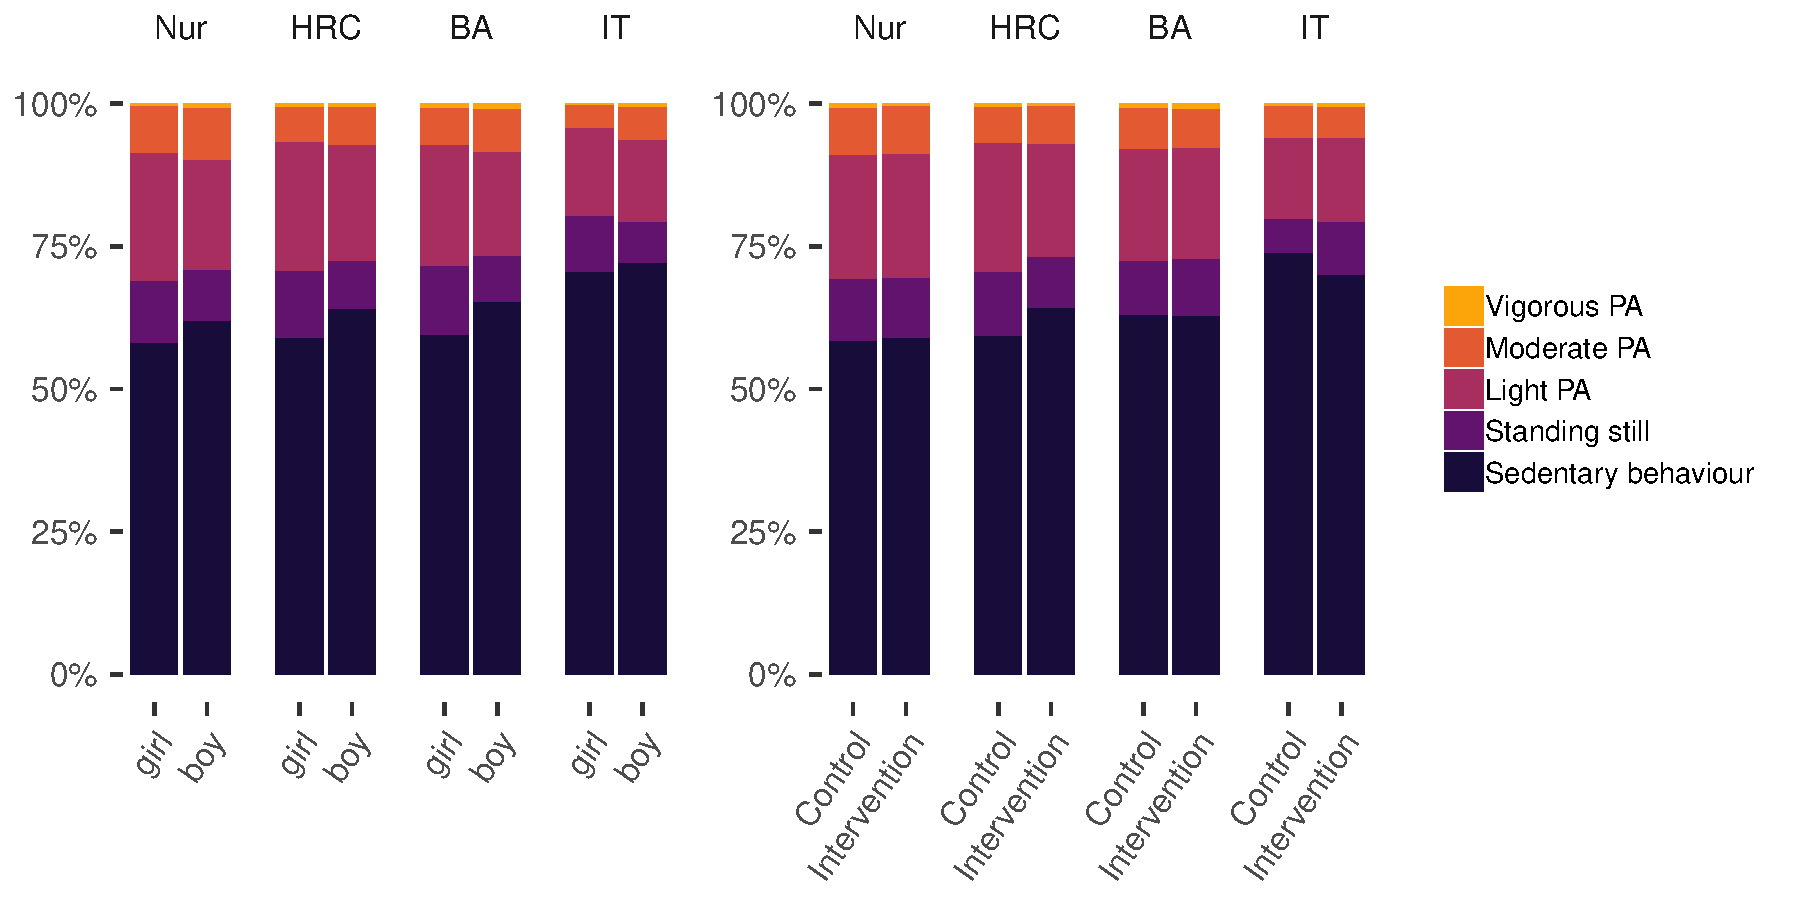
\includegraphics{_baseline-manuscript_files/figure-latex/average-day-activity-plot-1.pdf}
\caption{\label{fig:average-day-activity-plot}Averaged proportions of
activity during an average day.}
\end{figure}

The plot shows the averages aggregated across individuals and, while
being clear, hides variability in the activity types. For example, while
the average portion of the day spent in sedentary behaviour was 68\%,
almost every fourth (23\%) participant was sedentary more than 75\% of
the measurement time.

Figure \ref{fig:MVPA-accelerometer-sm} displays a density plot. It can
be read like a histogram, but the shape is not dependent on the bar
size, which is often set by software defaults and may not reflect the
research needs at hand. The density curve also helps illustrate
differences across groups.

\begin{verbatim}
## 
## Test of equal densities:  p-value =  0
## 
## Test of equal densities:  p-value =  0.09
\end{verbatim}

\begin{figure}
\centering
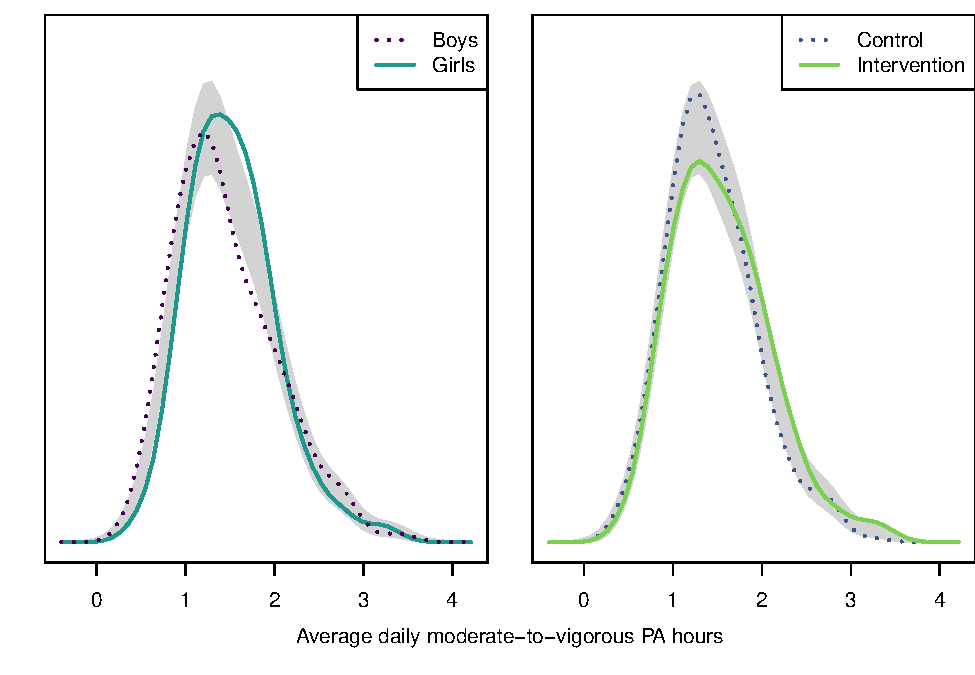
\includegraphics{_baseline-manuscript_files/figure-latex/MVPA-accelerometer-sm-1.pdf}
\caption{\label{fig:MVPA-accelerometer-sm}Accelerometer-measured MVPA
minutes. Grey region in depicts bootstrapped area of equivalence, given
independent observations. Figure implemented by R package sm.}
\end{figure}

We can see, that girls seem to be more active than boys, or more
specifically, there are more girls who reached an average of 1.5-2 hours
of MVPA, and less of them who were lower. Although the grey band does
not take clustering in classes, schools and educational tracks into
account, it provides a heuristic for determining divergences between
groups. Given that boys are generally more active than girls (P. Husu et
al., 2016), this warrants a closer inspection, as presented by the
density plots in figure \ref{fig:MVPA-accelerometer-plot}.

\begin{figure}
\centering
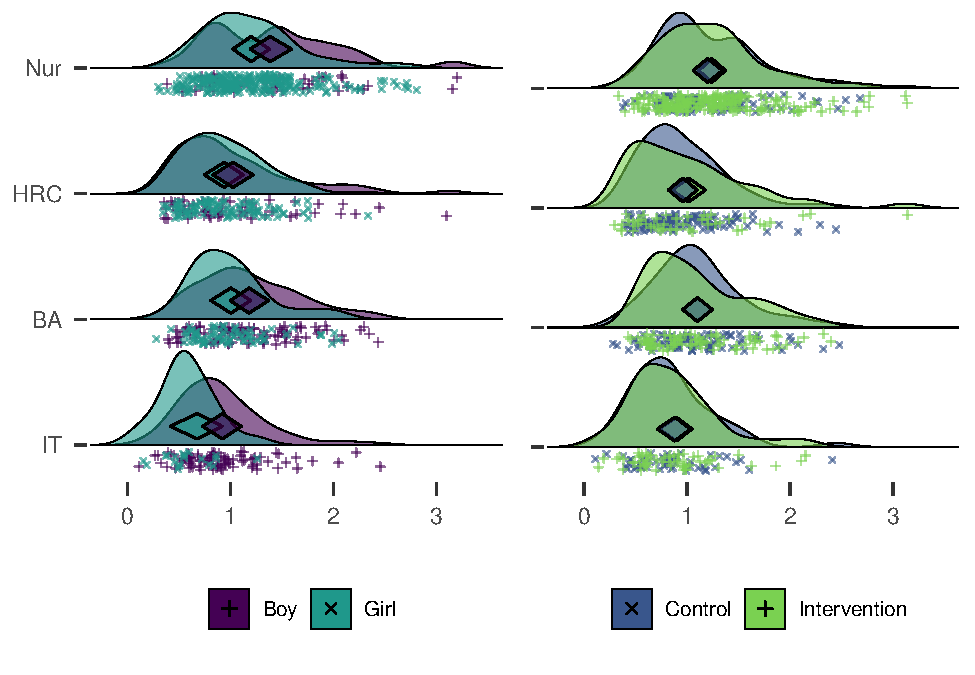
\includegraphics{_baseline-manuscript_files/figure-latex/MVPA-accelerometer-plot-1.pdf}
\caption{\label{fig:MVPA-accelerometer-plot}Hours of moderate-to-vigorous PA
for different educational tracks. Midpoints of diamonds indicate means,
endpoints 95\% credible intervals. Individual observations are presented
under the density curves, with random scatter on the y-axis to ease
inspection. Figure implemented by R package ggridges. Nur = Practical
nurse, HRC = Hotel, restaurant and catering, BA = Business and
administration, IT = Information and communications technology.}
\end{figure}

As can be seen from the x-axis placement of diamonds in figure
\ref{fig:MVPA-accelerometer-plot}, participants who study to be
practical nurses are the most active, followed by HRC students and BA
students, with the IT track being the least active, though there is
considerable variation within tracks. This also explains the difference
in MVPA among girls and boys: the practical nurse track is the largest,
and its students are most active, as well as mostly girls. The
information technology students are the least active, but mostly boys.

In sum, boys are slightly more active in most of the tracks (mean
differences---7.40 minutes for Practical nurse, -0.40 for Hotel,
restaurant and catering, 7.50 for Business and administration, and 17.10
for Information and communications technology---are small and can be
attributed to random variation). In spite of this, girls appear more
active in the aggregate. This is also known as the Simpson's paradox,
and is best approached by visualising data (see Kievit, Frankenhuis,
Waldorp, and Borsboom (2013) for an introduction).

\subsection{Self-reported MVPA}\label{self-reported-mvpa}

The number of days participants reported doing PA on, suggested a
different picture of difference between genders in activity.

Figure xxx. Self-reported frequency of MVPA. From figure xxx, we can see
that there were more boys reporting a high number of MVPA days, and
fewer boys reported low numbers. This effect was consistent among
educational tracks. Boys and girls, as well as different educational
tracks, differed largely in the types of PA they reported having engaged
in during the previous month (see supplement at \enquote{Types of
self-reported exercise}).

\subsection{Breaks in sedentary time}\label{breaks-in-sedentary-time}

Girls in all educational tracks interrupted sitting more than boys.

Figure xxx. Breaks in sedentary time.

\subsection{Time spent sitting and lying
down}\label{time-spent-sitting-and-lying-down}

Differences in time spent sitting and lying down emerged between boys
and girls, the former having more sedentary time. Even though there was
some heterogeneity among schools, again the aggregated intervention and
control schools showed no differences.

Breaking the distributions down by tracks, this is what we see:

Figure xxx. Average time spent sitting or lying down during a day. Nur =
Practical nurse, HRC = Hotel, restaurant and catering, BA = Business and
administration, IT = Information and communications technology.

Figure XXX shows, that boys are more sedentary in all groups, but the IT
group--which consists of mostly boys--is also most sedentary regardless
of gender. Distributions between intervention and control groups exhibit
some differences, but the most pronounced one can be seen in the HRC
track.

Figure \ref{fig:network-plot} shows the network model

\begin{figure}
\centering
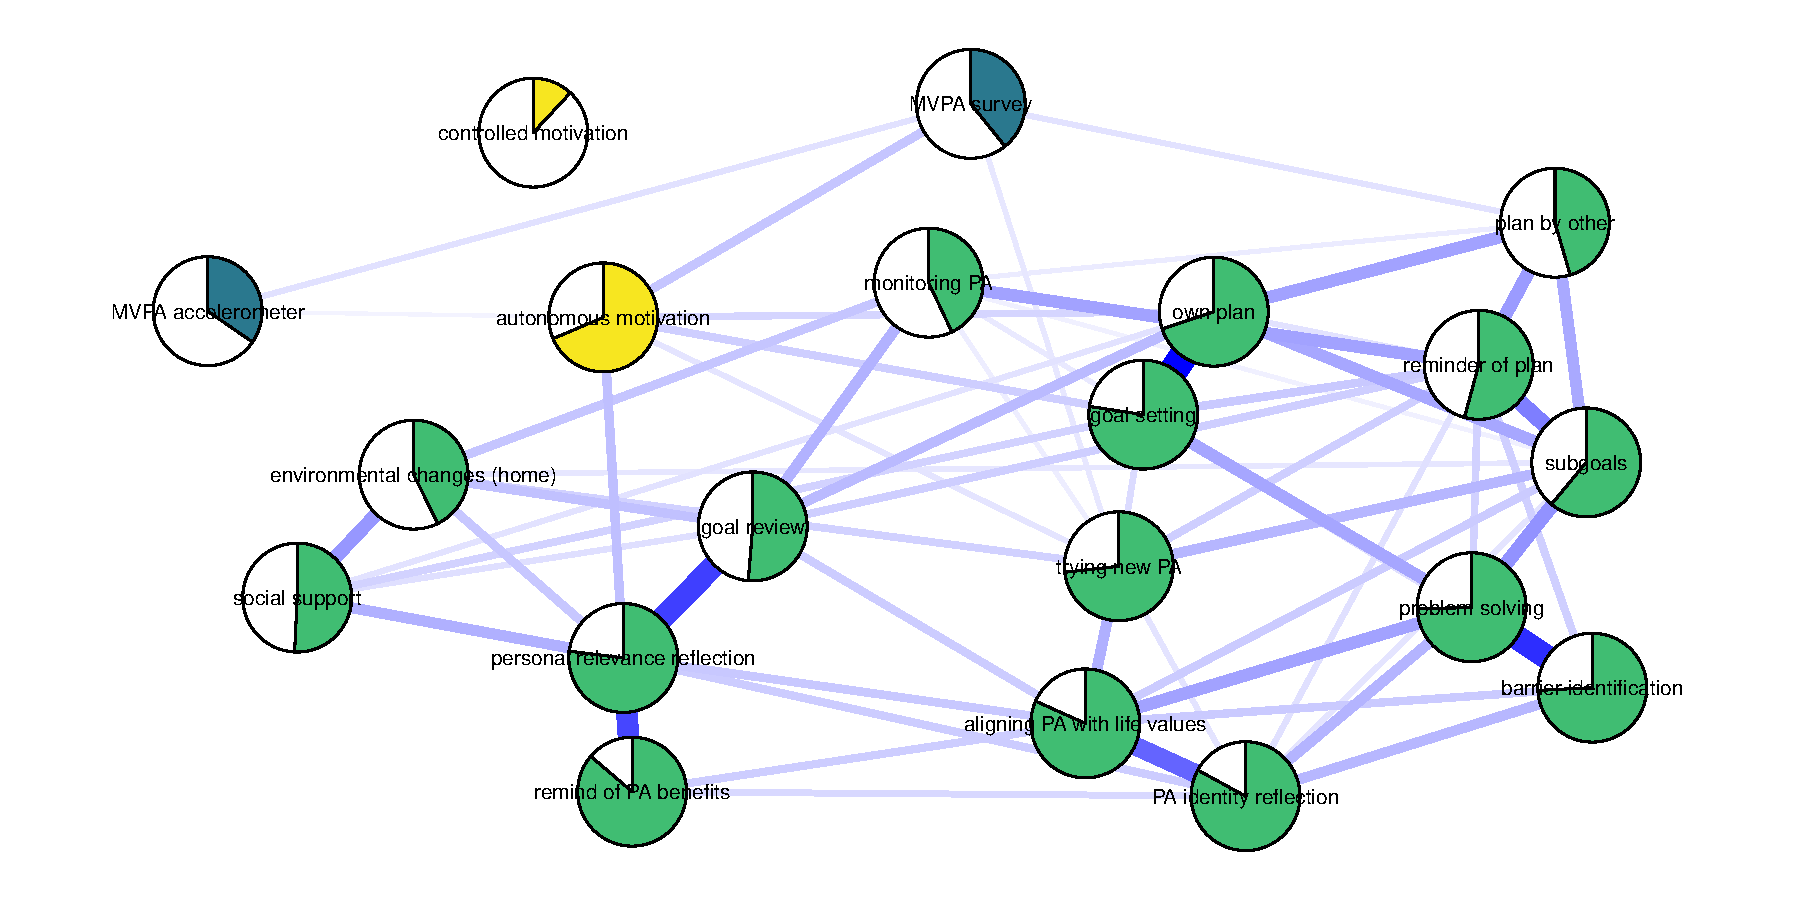
\includegraphics{_baseline-manuscript_files/figure-latex/network-plot-1.pdf}
\caption{\label{fig:network-plot}A) Mixed graphical model with LASSO
regularisation and model selection by cross-validation, B) Bivariate
correlation network}
\end{figure}

\newpage

\section{References}\label{references}

\begingroup
\setlength{\parindent}{-0.5in} \setlength{\leftskip}{0.5in}

\hypertarget{refs}{}
\hypertarget{ref-brigantiNetworkAnalysisEmpathy2018}{}
Briganti, G., Kempenaers, C., Braun, S., Fried, E. I., \& Linkowski, P.
(2018). Network analysis of empathy items from the interpersonal
reactivity index in 1973 young adults. \emph{Psychiatry Research},
\emph{265}, 87--92.
doi:\href{https://doi.org/10.1016/j.psychres.2018.03.082}{10.1016/j.psychres.2018.03.082}

\hypertarget{ref-costantiniStateARtPersonality2015}{}
Costantini, G., Epskamp, S., Borsboom, D., Perugini, M., Mõttus, R.,
Waldorp, L. J., \& Cramer, A. O. (2015). State of the aRt personality
research: A tutorial on network analysis of personality data in R.
\emph{Journal of Research in Personality}, \emph{54}, 13--29.
doi:\href{https://doi.org/10.1016/j.jrp.2014.07.003}{10.1016/j.jrp.2014.07.003}

\hypertarget{ref-costantiniStabilityVariabilityPersonality2017}{}
Costantini, G., Richetin, J., Preti, E., Casini, E., Epskamp, S., \&
Perugini, M. (2017). Stability and variability of personality networks.
A tutorial on recent developments in network psychometrics.
\emph{Personality and Individual Differences}.
doi:\href{https://doi.org/10.1016/j.paid.2017.06.011}{10.1016/j.paid.2017.06.011}

\hypertarget{ref-dalegeNetworkStructureExplains2017}{}
Dalege, J., Borsboom, D., Harreveld, F., Waldorp, L. J., \& Maas, H. L.
(2017). Network structure explains the impact of attitudes on voting
decisions. \emph{Scientific Reports}, \emph{7}(1), 4909.

\hypertarget{ref-dalegeNetworkAnalysisAttitudes2017}{}
Dalege, J., Borsboom, D., van Harreveld, F., \& van der Maas, H. L.
(2017). Network analysis on attitudes: A brief tutorial. \emph{Social
Psychological and Personality Science}, \emph{8}(5), 528--537.

\hypertarget{ref-dalegeFormalizedAccountAttitudes2016}{}
Dalege, J., Borsboom, D., van Harreveld, F., van den Berg, H., Conner,
M., \& van der Maas, H. L. J. (2016). Toward a formalized account of
attitudes: The Causal Attitude Network (CAN) model. \emph{Psychological
Review}, \emph{123}(1), 2--22.
doi:\href{https://doi.org/10.1037/a0039802}{10.1037/a0039802}

\hypertarget{ref-degrootMeaningSignificanceDifferent2014}{}
de Groot, A. D. (2014). The meaning of ``significance'' for different
types of research {[}translated and annotated by Eric-Jan Wagenmakers,
Denny Borsboom, Josine Verhagen, Rogier Kievit, Marjan Bakker, Angelique
Cramer, Dora Matzke, Don Mellenbergh, and Han L. J. van der Maas{]}.
\emph{Acta Psychologica}, \emph{148}, 188--194.
doi:\href{https://doi.org/10.1016/j.actpsy.2014.02.001}{10.1016/j.actpsy.2014.02.001}

\hypertarget{ref-dielemanTrendsFutureHealth2018}{}
Dieleman, J. L., Sadat, N., Chang, A. Y., Fullman, N., Abbafati, C.,
Acharya, P., \ldots{} Alizadeh-Navaei, R. (2018). Trends in future
health financing and coverage: Future health spending and universal
health coverage in 188 countries, 2016--40. \emph{The Lancet},
\emph{391}(10132), 1783--1798.

\hypertarget{ref-elgarSocioeconomicInequalitiesAdolescent2015}{}
Elgar, F. J., Pförtner, T.-K., Moor, I., De Clercq, B., Stevens, G. W.
J. M., \& Currie, C. (2015). Socioeconomic inequalities in adolescent
health 2002--2010: A time-series analysis of 34 countries participating
in the Health Behaviour in School-aged Children study. \emph{The
Lancet}, \emph{385}(9982), 2088--2095.
doi:\href{https://doi.org/10.1016/S0140-6736(14)61460-4}{10.1016/S0140-6736(14)61460-4}

\hypertarget{ref-epskampTutorialRegularizedPartial2018}{}
Epskamp, S., \& Fried, E. I. (2018). A Tutorial on Regularized Partial
Correlation Networks. \emph{Psychological Methods}.
doi:\href{https://doi.org/10.1037/met0000167}{10.1037/met0000167}

\hypertarget{ref-epskampEstimatingPsychologicalNetworks2016}{}
Epskamp, S., Borsboom, D., \& Fried, E. I. (2016). Estimating
Psychological Networks and their Stability: A Tutorial Paper.
\emph{arXiv Preprint arXiv:1604.08462}.

\hypertarget{ref-fagtNordicMonitoringDiet2012}{}
Fagt, S., Andersen, L. F., Anderssen, S. A., Becker, W., Borodulin, K.,
Fogelholm, M., \ldots{} Trolle, E. (2012). \emph{Nordic Monitoring of
diet, physical activity and overweight : Validation of indicators}.
Nordic Council of Ministers.

\hypertarget{ref-friedMentalDisordersNetworks2017}{}
Fried, E. I., van Borkulo, C. D., Cramer, A. O., Boschloo, L.,
Schoevers, R. A., \& Borsboom, D. (2017). Mental disorders as networks
of problems: A review of recent insights. \emph{Social Psychiatry and
Psychiatric Epidemiology}, \emph{52}(1), 1--10.

\hypertarget{ref-haigTestsStatisticalSignificance2016}{}
Haig, B. D. (2016). Tests of Statistical Significance Made Sound.
\emph{Educational and Psychological Measurement}.
doi:\href{https://doi.org/10.1177/0013164416667981}{10.1177/0013164416667981}

\hypertarget{ref-hankonenLetMoveIt2016}{}
Hankonen, N., Heino, M. T. J., Araujo-Soares, V., Sniehotta, F. F.,
Sund, R., Vasankari, T., \ldots{} Haukkala, A. (2016). ``Let's Move It''
a school-based multilevel intervention to increase physical activity and
reduce sedentary behaviour among older adolescents in vocational
secondary schools: A study protocol for a cluster-randomised trial.
\emph{BMC Public Health}, \emph{16}, 451--466.
doi:\href{https://doi.org/10.1186/s12889-016-3094-x}{10.1186/s12889-016-3094-x}

\hypertarget{ref-hankonenRandomisedControlledFeasibility2017}{}
Hankonen, N., Heino, M. T. J., Hynynen, S.-T., Laine, H.,
Ara\a'ujo-Soares, V., Sniehotta, F. F., \ldots{} Haukkala, A. (2017a).
Randomised controlled feasibility study of a school-based multi-level
intervention to increase physical activity and decrease sedentary
behaviour among vocational school students. \emph{International Journal
of Behavioral Nutrition and Physical Activity}, \emph{14}(1).
doi:\href{https://doi.org/10.1186/s12966-017-0484-0}{10.1186/s12966-017-0484-0}

\hypertarget{ref-hankonenWhatExplainsSocioeconomic2017}{}
Hankonen, N., Heino, M. T., Kujala, E., Hynynen, S.-T., Absetz, P.,
Ara\a'ujo-Soares, V., \ldots{} Haukkala, A. (2017b). What explains the
socioeconomic status gap in activity? Educational differences in
determinants of physical activity and screentime. \emph{BMC Public
Health}, \emph{17}(1), 144. Retrieved from
\url{https://bmcpublichealth.biomedcentral.com/articles/10.1186/s12889-016-3880-5}

\hypertarget{ref-husuObjectivelyMeasuredSedentary2016}{}
Husu, P., Vähä-Ypyä, H., \& Vasankari, T. (2016). Objectively measured
sedentary behavior and physical activity of Finnish 7-to 14-year-old
children--associations with perceived health status: A cross-sectional
study. \emph{BMC Public Health}, \emph{16}(1), 338.

\hypertarget{ref-hynynenSystematicReviewSchoolbased2016}{}
Hynynen, S.-T., van Stralen, M. M., Sniehotta, F. F., Ara\a'ujo-Soares,
V., Hardeman, W., Chinapaw, M. J. M., \ldots{} Hankonen, N. (2016). A
systematic review of school-based interventions targeting physical
activity and sedentary behaviour among older adolescents.
\emph{International Review of Sport and Exercise Psychology},
\emph{9}(1), 22--44.
doi:\href{https://doi.org/10.1080/1750984X.2015.1081706}{10.1080/1750984X.2015.1081706}

\hypertarget{ref-kievitSimpsonParadoxPsychological2013}{}
Kievit, R. A., Frankenhuis, W. E., Waldorp, L. J., \& Borsboom, D.
(2013). Simpson's paradox in psychological science: A practical guide.
\emph{Frontiers in Psychology}, \emph{4}.
doi:\href{https://doi.org/10.3389/fpsyg.2013.00513}{10.3389/fpsyg.2013.00513}

\hypertarget{ref-laiEstimatingStandardizedEffect2016}{}
Lai, M. H. C., \& Kwok, O.-m. (2016). Estimating Standardized Effect
Sizes for Two- and Three-Level Partially Nested Data. \emph{Multivariate
Behavioral Research}, \emph{51}(6), 740--756.
doi:\href{https://doi.org/10.1080/00273171.2016.1231606}{10.1080/00273171.2016.1231606}

\hypertarget{ref-laiFinitePopulationCorrection2018}{}
Lai, M. H., Kwok, O.-m., Hsiao, Y.-Y., \& Cao, Q. (2018). Finite
population correction for two-level hierarchical linear models.
\emph{Psychological Methods}, \emph{23}(1), 94.

\hypertarget{ref-lakensJustifyYourAlpha2018}{}
Lakens, D., Adolfi, F. G., Albers, C. J., Anvari, F., Apps, M. A. J.,
Argamon, S. E., \ldots{} Zwaan, R. A. (2018). Justify your alpha.
\emph{Nature Human Behaviour}, \emph{2}(3), 168--171.
doi:\href{https://doi.org/10.1038/s41562-018-0311-x}{10.1038/s41562-018-0311-x}

\hypertarget{ref-makelaPhysicalActivityScreen2016}{}
Mäkelä, K., Kokko, S., Kannas, L., Villberg, J., Vasankari, T.,
Heinonen, J. O., \ldots{} Selänne, H. (2016). Physical Activity, Screen
Time and Sleep among Youth Participating and Non-Participating in
Organized Sports: The Finnish Health Promoting Sports Club (FHPSC)
Study. \emph{Advances in Physical Education}, \emph{6}.

\hypertarget{ref-mooreProcessEvaluationComplex2015}{}
Moore, G. F., Audrey, S., Barker, M., Bond, L., Bonell, C., Hardeman,
W., \ldots{} Baird, J. (2015). Process evaluation of complex
interventions: Medical Research Council guidance. \emph{BMJ},
\emph{350}, h1258.
doi:\href{https://doi.org/10.1136/bmj.h1258}{10.1136/bmj.h1258}

\hypertarget{ref-mottusWhyTraitsCome2017}{}
Mõttus, R., \& Allerhand, M. (2017). Why do traits come together? The
underlying trait and network approaches. \emph{SAGE Handbook of
Personality and Individual Differences}, \emph{1}, 1--22.

\hypertarget{ref-nickersonNullHypothesisSignificance2000}{}
Nickerson, R. S. (2000). Null hypothesis significance testing: A review
of an old and continuing controversy. \emph{Psychological Methods},
\emph{5}(2), 241--301.
doi:\href{https://doi.org/http://dx.doi.org/10.1037/1082-989X.5.2.241}{http://dx.doi.org/10.1037/1082-989X.5.2.241}

\hypertarget{ref-nosekPreregistrationRevolution2018}{}
Nosek, B. A., Ebersole, C. R., DeHaven, A. C., \& Mellor, D. T. (2018).
The preregistration revolution. \emph{Proceedings of the National
Academy of Sciences}, 201708274.
doi:\href{https://doi.org/10.1073/pnas.1708274114}{10.1073/pnas.1708274114}

\hypertarget{ref-R-base}{}
R Core Team. (2018). \emph{R: A language and environment for statistical
computing}. Vienna, Austria: R Foundation for Statistical Computing.
Retrieved from \url{https://www.R-project.org/}

\hypertarget{ref-rstudioteamRStudioIntegratedDevelopment2016}{}
RStudio Team. (2016). RStudio: Integrated Development Environment for R.
Boston, MA: RStudio, Inc.

\hypertarget{ref-simmonsFalsePositivePsychologyUndisclosed2011}{}
Simmons, J. P., Nelson, L. D., \& Simonsohn, U. (2011). False-Positive
Psychology Undisclosed Flexibility in Data Collection and Analysis
Allows Presenting Anything as Significant. \emph{Psychological Science},
\emph{22}(11), 1359--1366.
doi:\href{https://doi.org/10.1177/0956797611417632}{10.1177/0956797611417632}

\hypertarget{ref-tibshiraniRegressionShrinkageSelection1996}{}
Tibshirani, R. (1996). Regression shrinkage and selection via the lasso:
A retrospective. \emph{Journal of the Royal Statistical Society: Series
B (Statistical Methodology)}, \emph{73}(3), 273--282.
doi:\href{https://doi.org/10.1111/j.1467-9868.2011.00771.x}{10.1111/j.1467-9868.2011.00771.x}

\hypertarget{ref-tremblaySedentaryBehaviorResearch2017}{}
Tremblay, M. S., Aubert, S., Barnes, J. D., Saunders, T. J., Carson, V.,
Latimer-Cheung, A. E., \ldots{} Chinapaw, M. J. (2017). Sedentary
Behavior Research Network (SBRN) process and outcome.
\emph{International Journal of Behavioral Nutrition and Physical
Activity}, \emph{14}, 75.
doi:\href{https://doi.org/10.1186/s12966-017-0525-8}{10.1186/s12966-017-0525-8}

\hypertarget{ref-vandermaasNetworkModelsCognitive2017}{}
Van Der Maas, H., Kan, K.-J., Marsman, M., \& Stevenson, C. E. (2017).
\emph{Network Models for Cognitive Development and Intelligence}.
Preprint.

\hypertarget{ref-vansluijsPhysicalActivityDietary2008}{}
van Sluijs, E. M., Skidmore, P. M., Mwanza, K., Jones, A. P., Callaghan,
A. M., Ekelund, U., \ldots{} Wareham, N. J. (2008). Physical activity
and dietary behaviour in a population-based sample of British 10-year
old children: The SPEEDY study (Sport, Physical activity and Eating
behaviour: Environmental Determinants in Young people). \emph{BMC Public
Health}, \emph{8}(1), 388.

\hypertarget{ref-vaha-ypyaReliableRecognitionLying2018}{}
VÃ\textcurrencyhÃ\textcurrency-YpyÃ\textcurrency, H., Husu, P., Suni,
J., Vasankari, T., \& Sievänen, H. (2018). Reliable recognition of
lying, sitting, and standing with a hip-worn accelerometer.
\emph{Scandinavian Journal of Medicine \& Science in Sports},
\emph{28}(3), 1092--1102.
doi:\href{https://doi.org/10.1111/sms.13017}{10.1111/sms.13017}

\hypertarget{ref-vaha-ypyaValidationCutpointsEvaluating2015}{}
VÃ\textcurrencyhÃ\textcurrency-YpyÃ\textcurrency, H., Vasankari, T.,
Husu, P., Mänttäri, A., Vuorimaa, T., Suni, J., \& Sievänen, H. (2015a).
Validation of cut-points for evaluating the intensity of physical
activity with accelerometry-based mean amplitude deviation (MAD).
\emph{PLoS One}, \emph{10}(8), e0134813.

\hypertarget{ref-vaha-ypyaUniversalAccurateIntensitybased2015}{}
VÃ\textcurrencyhÃ\textcurrency-YpyÃ\textcurrency, H., Vasankari, T.,
Husu, P., Suni, J., \& Sievänen, H. (2015b). A universal, accurate
intensity-based classification of different physical activities using
raw data of accelerometer. \emph{Clinical Physiology and Functional
Imaging}, \emph{35}(1), 64--70.

\endgroup






\end{document}
